\documentclass[./main.tex]{subfiles}

\begin{document}

\subsection{Purpose}

\textbf{SafeStreets} is a crowd-sourced application that intends to
provide users with the possibility to notify authorities when traffic
violations occur. The main target of the application are violations that
can be easily captured by a camera (like, for instance, parking
violations). SafeStreets intends also to provide users with the
possibility to mine the stored information with different levels of
visibility. Moreover, the application must cross the collected data with
information coming from the municipality to provide suggestions on
possible interventions to decrease the incidence of violations and
accidents. In the end, the application must forward data about
violations to generate traffic tickets, and must allow authorities to
get statistics on issued tickets.
\medskip\\
These requirements are exploited by developing several services:
\begin{itemize}
\item
  \textbf{SafeReports} allows common users to send violation reports.
\item
  \textbf{SafeAnalytics} allows common users and authorities to mine
  stored information.
\item
  \textbf{SafeTickets} allows authorities to get statistics on issued
  tickets.
\item
  \textbf{SafeSuggestions} allows municipality users to get suggestions
  on possible interventions.
\end{itemize}

\subsubsection{Goals}

The purpose of the software is captured by the following goals:
\begin{itemize}
\item
  \textbf{G1} SafeReports must allow common users to send violation
  reports.
\item
  \textbf{G2} SafeAnalytics must allow common users to get anonymous
  data on violations.
\item
  \textbf{G3} SafeAnalytics must allow authorities to access to all the
  data without restrictions.
\item
  \textbf{G4} SafeSuggestions must allow municipality users to get
  suggestions on possible interventions.
\item
  \textbf{G5} SafeStreets must generate traffic tickets forwarding
  reliable data to MTS.
\item
  \textbf{G6} SafeTickets must allow authorities to get statistics on
  issued tickets.
\end{itemize}

\subsection{Scope}

SafeStreets must interface with different types of users and information
sources. In this context, it is very important to identify the placement
of SafeStreets and its services with the entities of the scenario. To do
so, we will refer to the following picture. Afterward, every link
between SafeStreets and the entities will be deeply analyzed to
exhaustively describe the shared phenomena of the scenario.

\begin{figure}[H]
\centering
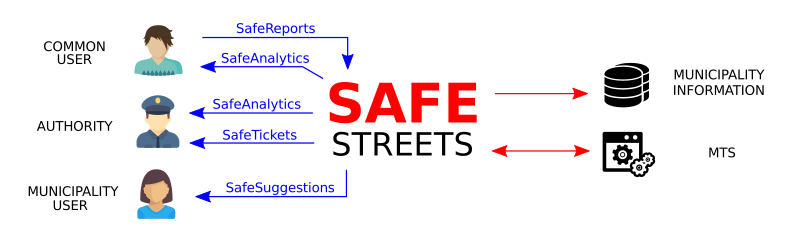
\includegraphics[width=\textwidth]{relationship_diagram}
\caption{Relationship diagram}
\end{figure}

Two types of interactions can be defined:
\begin{itemize}
\item
  \textbf{Interactions through services} (blue arrows in the diagram)
\item
  \textbf{Interactions with resources} (red arrows in the diagram)
\end{itemize}

The main difference between the interactions is the role of SafeStreets.
In the interactions through services, SafeStreets has a
passive role, in the sense that the activation of the interaction is
triggered by a request coming from the user through one of the offered
services. In the interactions with resources, SafeStreets has an active
role, in the sense that the activation of the interaction is
automatically triggered by SafeStreets application to exploit back-end
processes.
\medskip\\
Services are exploited differently depending on the type of user that is
enjoying the application. The type of the user is determined in the
registration phase, which is different depending on this choice.
Everyone can sign up as a common user. Instead, to sign up as an
authority or municipality user, it is necessary to provide a unique
disposable code, which assignment is not part of the application
(SafeStreets must take care only of the verification of the provided
code). The code is assigned only to users whose role declaration has
been manually verified by a human operator. For this reason, the
verification of authorities and municipality users is not considered in
the registration phase.

\subsubsection{SafeReports}

SafeReports is the core of the application. It provides common users
with the possibility to send a notification about a violation. To do so,
they are asked to take a picture of the vehicle involved in the
violation. Then the photo is checked and matched with some data captured
at the moment (position, date and time). The user is asked to review and
confirm the violation report that, in case of confirmation, is sent to
SafeStreets, which stores it to offer several other services.

\subsubsection{SafeAnalytics}

SafeAnalytics provides the possibility to mine SafeStreets data to get
information about violations. This service is offered to common users
and authorities, that can access data with different restriction levels.
Common users have access to anonymous data concerning a selected zone.
Authorities, instead, have access to unrestricted information on all the
stored data.

\subsubsection{SafeTickets}

SafeStreets uses Municipality Tickets Service (MTS) to generate traffic
tickets. When a new violation is stored (after it is verified not to be
a duplicated event), the violation report is forwarded to MTS which
generates the traffic tickets and informs SafeStreets of the outcome.
SafeStreets stores data about the issued tickets to provide statistics
through SafeTickets service.\\
SafeTickets is a service that allows authorities to access data about
tickets generated from SafeStreets using MTS. Authorities are also
allowed to select some filters to get statistics and aggregated data.

\subsubsection{SafeSuggestions}

Municipality data about accidents is crossed with data collected by
SafeStreets to identify possible unsafe areas and provide suggestions
through SafeSuggestions service. SafeStreets periodically checks for new
data to collect it and keep suggestions up to date.\\
SafeSuggestions service is developed to municipality users. It allows
them to access suggestions on how to reduce the accidents and violations
rate in the most critical zones. Users can ask for suggestions using
specific filters, depending on their intention to attend in a specific
zone or to prevent a specific violation.

\subsubsection{Shared phenomena}

\begin{table}[H]
\centering
\begin{tabularx}{\textwidth}{|X|l|l|}
\hline
Phenomenon & Shared & Controller\tabularnewline
\hline
A user wants to notify about a violation & No & World\tabularnewline
The user takes a picture using the application & Yes &
World\tabularnewline
The application scans the picture to find a license plate & No &
Machine\tabularnewline
The application does not find a license plate & No &
Machine\tabularnewline
The application asks the user to repeat the procedure & Yes &
Machine\tabularnewline
The application finds a license plate & No & Machine\tabularnewline
The application builds a violation report detecting position and
timestamp & No & Machine\tabularnewline
The application asks confirmation to the user & Yes &
Machine\tabularnewline
The user confirms the violation report & Yes & World\tabularnewline
The application stores the violation report & No &
Machine\tabularnewline
A user wants information on a violation & No & World\tabularnewline
The user selects certain filters & Yes & World\tabularnewline
An authority wants information on issued tickets & No &
World\tabularnewline
The authority selects certain filters & Yes & World\tabularnewline
The application searches for the requested data & No &
Machine\tabularnewline
The application returns and shows the requested data & Yes &
Machine\tabularnewline
A municipality user wants suggestions & No & World\tabularnewline
The municipality user select certain filters & Yes &
World\tabularnewline
The application searches for the requested suggestions & No &
Machine\tabularnewline
The application returns and shows the requested suggestions & Yes &
Machine\tabularnewline
The application forwards report violations to MTS * & Yes &
Machine\tabularnewline
The application stores data about issued tickets & No &
Machine\tabularnewline
The application requests data about accidents to the municipality * &
Yes & Machine\tabularnewline
The application stores data about accidents & No &
Machine\tabularnewline
The application analyzes data to identify suggestions & No &
Machine\tabularnewline
\hline
\end{tabularx}
\end{table}

* MTS and Municipality are considered part of the world, as they are not
part of the software to be.

\subsection{Definitions and acronyms}

\begin{itemize}
\item
  \textbf{User}\\
  The consumer of the application. It includes common users, authorities
  and municipality users.
\item
  \textbf{Common user}\\
  The user type that everyone can sign up as. It does not require any
  kind of verification.
\item
  \textbf{Authority}\\
  The user type that authorities can get. It requires the verification
  of an activation code.
\item
  \textbf{Municipality user}\\
  The user type that municipal employees can get. It requires the
  verification of an activation code.
\item
  \textbf{Timestamp}\\
  A set of information about the time. It includes date (day, month,
  year) and time (hour, minute, time zone).
\item
  \textbf{Violation report}\\
  The unit of notification collected by SafeStreets. It consists of:

  \begin{itemize}
  \item
    The picture of the violation
  \item
    The license plate of the vehicle involved
  \item
    The type of the violation
  \item
    The position of the violation
  \item
    The timestamp of the notification
  \end{itemize}
\item
  \textbf{Equivalent events}\\
  Set of violation reports that satisfy the following conditions:

  \begin{itemize}
  \item
    Same vehicles involved
  \item
    Same types of violation
  \item
    Position of the violations are different at most for 10 meters
  \item
    Same dates of the violations
  \end{itemize}
\item
  \textbf{Activation code}\\
  The code to be provided during the registration to get special permits
  on the account.
\item
  \textbf{Municipality Tickets Service (MTS)}\\
  Service offered by the municipality to generate traffic tickets from
  information about the violations.
\item
  \textbf{Optical Character Recognition (OCR)}\\
  Software that converts text scanned from a photo in a machine-encoded
  text.
\item
  \textbf{Query interface}\\
  The interface provided to the users to select some filters when
  requesting data.
\item
  \textbf{Application Programming Interface (API)}\\
  An interface or communication protocol between client and server
  intended to simplify the building of client-side software.
\end{itemize}

\subsection{Revision history}

\begin{table}[H]
\centering
\begin{tabularx}{0.9\textwidth}{|c|c|X|}
\hline
Version & Release date & Description\tabularnewline
\hline
1.0 & November 10, 2019 & First release\tabularnewline
1.1 & December 9, 2019 & Updated document formatting and added some comments
to clarify several concepts\tabularnewline
\hline
\end{tabularx}
\end{table}

\subsection{Document Structure}

\textbf{Section \ref{introduction}} is an overall introduction to the
application. It includes the description of the main functionalities of the
application, an analysis of scenarios in which the application works, the list
of the potential users of the application with a concise description of the
possible interactions and the definition of world-level goals. Also,
some meta-information is included, like revision history, references,
and explanation of the conventions occurring in the document.
\medskip\\
\textbf{Section \ref{overall_description}} includes the domain assumptions, a
detailed description of the shared phenomena and a formal description of the
domain carried out using UML class and state diagrams. The purpose of
this section is to exhaustively describe the entities and the scenarios
that the application must interact with, to be able, in the following
sections, to focus only on the application requirements.
\medskip\\
\textbf{Section \ref{specific_requirements}} includes a detailed description of
the application, useful for the development team. Here are classified the
interfaces offered by the application, followed by requirements and
constraints. More specifically, requirements are listed and matched with the
domain assumptions to show how every goal is attained. In this section, the
behavior of the application is described with the highest detail level
through the use of sequence, activity, and use case diagrams.
\medskip\\
\textbf{Section \ref{formal_analysis_using_alloy}} includes the formal analysis
carried out using Alloy as a modeling language. This section includes the model
built focusing on the most critical aspects and the results of the analysis
that proves the soundness and consistency of the model. Moreover, some worlds
obtained by running the analysis are included to study in deep the most
meaningful assertions.
\medskip\\
\textbf{Section \ref{effort_spent}} includes information about the number of
hours each group member has worked for this document.
\medskip\\
\textbf{Section \ref{references}} includes the references to the tools used to
draw up this document.

\end{document}